\documentclass[a4paper,11pt]{article}
\usepackage{graphicx}
\usepackage{graphicx}
\usepackage[margin=2.5cm]{geometry}
\usepackage[utf8]{inputenc}
\usepackage{float}
%\usepackage[T1]{fontenc}
\usepackage[czech]{babel}
\usepackage[justification=centering,labelfont=bf]{caption}
\usepackage{listings}
\graphicspath{{Images/}}
\usepackage{color}
\usepackage{caption}
\usepackage{fancyhdr}
\usepackage{tikz}
\usepackage{fontspec}
\usepackage{hyperref}
%\usepackage{framed}
\usetikzlibrary{shapes.geometric, arrows.meta, positioning, calc}

\usepackage[backend=biber,style=numeric]{biblatex}
\addbibresource{refs.bib}

\hypersetup{
	colorlinks,
	linkcolor={blue!100!black},
	citecolor={blue!100!black},
	urlcolor={blue!80!black}
}

\lstset{language=python}
\lstset{literate= {á}{{\'a}}1 {é}{{\'e}}1 {í}{{\'i}}1 {ó}{{\'o}}1 {ú}{{\'u}}1 {ý}{{\'y}}1 {č}{{\v{c}}}1 {ď}{{\v{d}}}1 {ě}{{\v{e}}}1 {ň}{{\v{n}}}1 {ř}{{\v{r}}}1 {š}{{\v{s}}}1 {ť}{{\v{t}}}1 {ů}{{\r{u}}}1 {ž}{{\v{z}}}1 {Á}{{\'A}}1 {É}{{\'E}}1 {Í}{{\'I}}1 {Ó}{{\'O}}1 {Ú}{{\'U}}1 {Ý}{{\'Y}}1 {Č}{{\v{C}}}1 {Ď}{{\v{D}}}1 {Ě}{{\v{E}}}1 {Ň}{{\v{N}}}1 {Ř}{{\v{R}}}1 {Š}{{\v{S}}}1 {Ť}{{\v{T}}}1 {Ů}{{\r{U}}}1 {Ž}{{\v{Z}}}1}


\definecolor{codegreen}{rgb}{0,0.6,0}
\definecolor{codegray}{rgb}{0.5,0.5,0.5}
\definecolor{codepurple}{rgb}{0.58,0,0.82}
\definecolor{backcolour}{rgb}{0.95,0.95,0.92}

\lstdefinestyle{mystyle}{
    backgroundcolor=\color{backcolour},   
    commentstyle=\color{codegreen},
    keywordstyle=\color{magenta},
    numberstyle=\tiny\color{codegray},
    stringstyle=\color{codepurple},
    basicstyle=\ttfamily\footnotesize,
    breakatwhitespace=false,         
    breaklines=true,                 
    captionpos=b,                    
    keepspaces=true,                 
    numbers=left,                    
    numbersep=5pt,                  
    showspaces=false,                
    showstringspaces=false,
    showtabs=false,                  
    tabsize=2
}
\lstset{style=mystyle}

\pagestyle{fancy}
\fancyhf{}
\lhead{Gymnázium Arabská 14, Praha 6}
\rhead{\small\textbf{RHEED}}

\rfoot{\thepage}

\begin{document}
	\thispagestyle{empty}
	
	\begin{flushleft}
		
\includegraphics[width=2cm]{logo.png}
		\begin{tabular}[b]{@{}p{0.6\textwidth}}
			\large\textbf{Gymnázium, Praha 6, Arabská 14}\\
			\textbf{Předmět:} Programování\\
			\textbf{Vedoucí práce:} Ing. Daniel Kahoun\\
			\textbf{Odborná konzultace:} Dr. Dominik Kriegner, Ing. Filip Křížek, Ph. D. 
		\end{tabular}
	\end{flushleft}
	
	\begin{center}
		\vspace{1cm}
		{\Huge\textbf{Aplikace pro vizualizaci a analýzu dat z in-situ měření RHEED při epitaxi monoatomárních vrstev pomocí technologie MBE}}\\
		\vspace{0.5cm}
		Ročníková práce
		\vspace{0.5cm}
	\end{center}
	
	\begin{figure}[H]
		\centering
		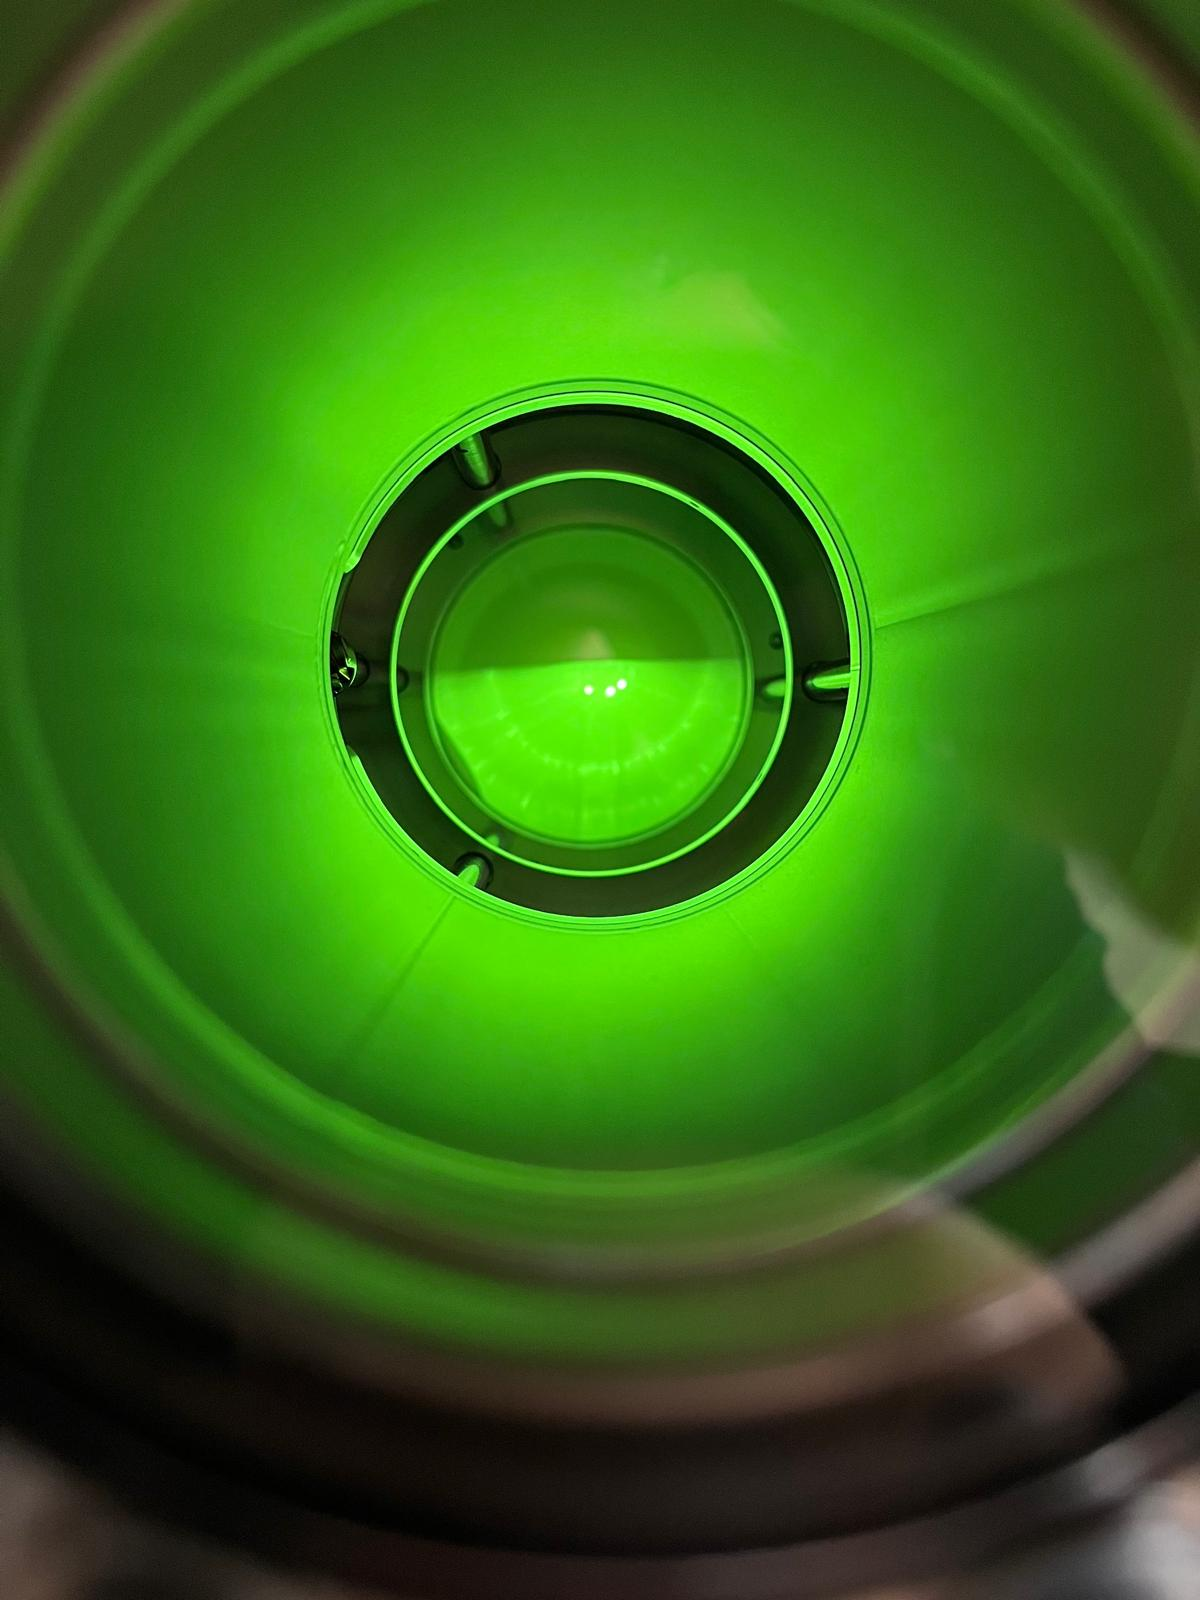
\includegraphics[width=0.45 \textwidth]{title.png}
	\end{figure}

	
	\begin{flushleft}
		Marek Bílý\\
		Marek Švec\\
		Jan Schreiber
		\hspace{11cm}
		březen 2024\\
	\end{flushleft}
	
	\newpage
	\thispagestyle{empty}
	\section*{Prohlášení}
Prohlašujeme, že jsme jedinými autory tohoto projektu, všechny citace jsou
řádně označené a všechna použitá literatura a další zdroje jsou v práci uvedeny.

Tímto dle zákona 121/2000 Sb. (tzv. Autorský zákon) ve znění pozdějších předpisů udělujeme
bezúplatně škole Gymnázium, Praha 6, Arabská 14 oprávnění k výkonu práva na rozmnožování díla
(§ 13) a práva na sdělování díla veřejnosti (§ 18) na dobu časově neomezenou a bez omezení
územního rozsahu.

\vspace{1.5cm}

\noindent
\begin{tabular}{l c}
    Podpis autora: & \makebox[6cm]{\hrulefill} \\
    \vspace{0.8cm} \\
    Podpis autora: & \makebox[6cm]{\hrulefill} \\
    \vspace{0.8cm} \\
    Podpis autora: & \makebox[6cm]{\hrulefill} \\
\end{tabular} 
\hfill
\begin{tabular}{r}
    Datum: \makebox[3cm]{\hrulefill} \\
\end{tabular}

\newpage
\pagenumbering{arabic}
\pagestyle{fancy}

\tableofcontents
\newpage


\section{Slovník}
\begin{itemize}
\item \textbf{RHEED – Reflection High-Energy Electron Diffraction} - metoda povrchové analýzy krystalických materiálů.\\
\item \textbf{CCD – Charge-Coupled Device} - zařízení pro detekci a záznam obrazu.\\
\item \textbf{MBE – Molecular Beam Epitaxy} - metoda epitaxního růstu tenkých vrstev.\\
\item \textbf{OpenGL – Open Graphics Library} - knihovna pro vykreslování 2D a 3D grafiky pomocí GPU.\\
\item \textbf{ROI – Region of Interest} - oblast zájmu v obraze určená pro detailní analýzu.\\
\item \textbf{HDF5 – Hierarchical Data Format version 5} - formát pro strukturované ukládání velkých dat.\\
\item \textbf{XRD – X-ray Diffraction} - rentgenová difrakční metoda pro analýzu krystalové struktury.\\
\item \textbf{STM – Scanning Tunneling Microscopy} - rastrovací tunelová mikroskopie pro analýzu povrchů na atomární úrovni.\\
\item \textbf{GUI – Graphical User Interface} - grafické uživatelské rozhraní.\\
\item \textbf{Toolbar – nástrojová lišta} - Toolbar obsahuje tlačítka pro rychlý přístup k funkcím aplikace, jako je navigace, úprava obrazu nebo analýza dat.
\end{itemize}
\newpage

\section*{Anotace}

\subsection*{Název práce: Aplikace pro vizualizaci a analýzu dat z in-situ měření RHEED při epitaxi monoatomárních vrstev pomocí technologie MBE}
autoři: Marek Bílý, Jan Schreiber, Marek Švec
\vspace{0.5cm}

Tato práce se zabývá vývojem softwaru pro analýzu a vizualizaci obrazových dat získaných metodou RHEED. RHEED je významná analytická metoda využívaná ve fyzice pevných látek, která umožňuje detailní studium povrchové struktury materiálů během epitaxního růstu. Cílem práce je vytvořit efektivní aplikaci, která umožní snímání, zpracování a analýzu difrakčních obrazců v reálném čase. Tato analýza bude výsledně nápomocná při růstu MBE na různých vědeckých pracovištích s primárním využitím na vědeckých pracovištích Fyzikálního ústavu AV ČR a to na oddělení spintroniky a kvantových materiálů Dr. Jungwirtha a ve výzkumné skupině Dr. Tima Verhagena zabývající se přípravou sandwichových materiálů s feroelektrickými vlastnostmi.

\subsection*{Title: Application for Visualization and Analysis of Data from In-Situ RHEED Measurements during the Epitaxy of Monolayers Using MBE Technology}
authors: Marek Bílý, Jan Schreiber, Marek Švec
\vspace{0.5cm}

This work is focused on the development of software for the analysis and visualization of image data acquired using the RHEED method. RHEED is an important analytical technique employed in solid state physics that enables a detailed study of the surface structure of materials during epitaxial growth. The objective of this work is to create an effective application that facilitates the capturing, processing, and real-time analysis of diffraction patterns. Ultimately, this analysis will support MBE growth at various scientific institutions, with primary usage at the Institute of Physics, Academy of Sciences of the Czech Republic – specifically within the department of spintronics and quantum materials under Dr. Jungwirth, and in the research group of Dr. Tim Verhagen, which is engaged in the preparation of sandwich materials with ferroelectric properties.

\subsection*{Titel: Anwendung zur Visualisierung und Analyse von Daten aus in-situ RHEED-Messungen bei der Epitaxie von Monoschichten unter Einsatz der MBE-Technologie}
Autoren: Marek Bílý, Jan Schreiber, Marek Švec
\vspace{0.5cm}

Diese Arbeit befasst sich mit der Entwicklung einer Software zur Analyse und Visualisierung von Bilddaten, die mittels der RHEED-Methode gewonnen wurden. RHEED ist eine bedeutende analytische Technik in der Festkörperphysik, die eine detaillierte Untersuchung der Oberflächenstruktur von Materialien während des epitaktischen Wachstums ermöglicht. Ziel dieser Arbeit ist es, eine effektive Anwendung zu entwickeln, die das Erfassen, Verarbeiten und die Echtzeitanalyse von Beugungsmustern ermöglicht. Letztlich soll diese Analyse das MBE-Wachstum an verschiedenen wissenschaftlichen Einrichtungen unterstützen, wobei der primäre Einsatzort das Institut für Physik der Akademie der Wissenschaften der Tschechischen Republik ist – insbesondere in der Abteilung für Spintronik und Quantenmaterialien unter der Leitung von Dr. Jungwirth sowie in der Forschungsgruppe von Dr. Tim Verhagen, die sich mit der Herstellung von Sandwichmaterialien mit ferroelektrischen Eigenschaften beschäftigt.
\newpage

\section{Úvod}
    RHEED je metoda povrchové analýzy krystalických materiálů. Je zde využíván vysokoenergetický elektronový paprsek, který pod velmi malým úhlem dopadá na krystalickou strukturu zkoumaného materiálu. Elektrony se následně odrážejí od atomů na povrchu a vytvářejí tzv. difrakční vzor. Ten obsahuje potřebné informace o vzorku.\\

    RHEED se skládá ze tří hlavních komponent: zdroje elektronového paprsku, vzorku a detekčního systému. Zdroj elektronového paprsku, někdy nazývaný elektronové dělo, je zodpovědný za generování vysokoenergetického svazku přesně zamířeného na povrch krystalového vzorku. Vzorek je umístěn v ultravysokém vakuu například v růstové komoře epitaxního nanášecího systému, kde lze se vzorkem pomocí otáčecího stolku manipulovat. Detekční systém má za úkol zachycovat difrakční vzor vzniklý rozptýlením elektronů po střetu s atomy vzorku. Nejběžnějšími nástroji zde slouží fluorescenční obrazovka (scintilátor), na kterou dopadají zmíněné elektrony, a CCD kamera, která obraz zaznamenává. K analýze sebraných dat nakonec slouží softwarový program, jehož vytvoření je cílem naší práce. Výsledné difrakční vzory následně umožňují hlubší porozumění v jaké fázi růstu se proces nachází, kolik monoatomárních vrstev již bylo na vzorek deponováno, v jaké kvalitě, aj.
    
\subsection{Zadání a cíl práce}
    Aplikace bude sloužit jako lepší alternativa stávající, z části nefunkční, aplikace v jazyce C\#. Vývoj bude obsahovat jak hardware interfacing s CCD detektorem, návrh a realizaci GUI, práci s obrazovými daty z kamery, vizualizaci real-time a analýzu real-time obrazových dat a ukládání starších měřených dat do vhodného datového typu pro další výzkum. Aplikace bude využívat in-situ měřící metodu RHEED snímající difrakční vzory vysokoenergetických elektronů při odrazu od povrchu vzorků. Zpracování dat z této metody bude sloužit k charakterizaci celého procesu a spolehlivější predikci výsledku růstu ještě před jeho dokončením. 
    
    Výsledný program bude mít potenciální využití na vědeckých pracovištích Fyzikálního ústavu AV ČR a to na oddělení spintroniky a kvantových materiálů Dr. Jungwirtha a ve výzkumné skupině Dr. Tima Verhagena zabývající se přípravou sandwichových materiálů s feroelektrickými vlastnostmi.
    
\subsection{Odborná konzultace a projektování ve spolupráci s pracovníky FZÚ}
	Po celou dobu vypracovávání práce byla velice klíčovou úzká spolupráce s odborníky z Fyzikálního ústavu AV ČR a to především: \textbf{Dr. Dominikem Kriegnerem a Ing. Filipem Křížkem, Ph. D.} Díky této spolupráci jsme byli schopni vyhovět všem požadavkům a nárokům na aplikaci během praktického využití při výzkumných činnostech na ústavu. Tohoto jsme docílili za pomoci pravidelných osobních schůzek na FZÚ a vedením a dokumentace připomínek
	
	
\newpage
\subsection{Použité technologie}

Pro realizaci projektu byly využity následující knihovny:

\begin{itemize}
    \item \textbf{h5py (3.13.0)} – Knihovna pro práci se soubory ve formátu HDF5, využívaná pro ukládání a organizaci obrazových dat. 
    \item \textbf{matplotlib (3.10.0)} – Vizualizace dat v Pythonu.
    \item \textbf{numpy (2.2.3)} – Vědecké výpočty a efektivní práce s poli.
    \item \textbf{opencv (4.11.0.86)} – Zpracování obrazu a práci s kamerou.
    \item \textbf{OpenGL} – Rozhraní pro 2D a 3D grafiku.
    \item \textbf{PyQt5 (5.15.11)} – Tvorbu GUI na bázi Qt.
    \item \textbf{dateutil (2.9.0)} – Rozšíření práce s datem a časem.
    \item \textbf{silx (2.2.0 a 1.17.0)} – Vědecké vizualizace a práce s daty.
\end{itemize}

Kromě těchto knihoven byly při vývoji softwaru využity i další nástroje, zejména:

\begin{itemize}
    \item \textbf{Python 3.10+} – Hlavní programovací jazyk projektu.
    \item \textbf{Visual Studio Code} – Vývojové prostředí používané pro programování a ladění kódu.
    \item \textbf{Player One Saturn-C} – Kamera použitá pro sběr difrakčních snímků.
\end{itemize}

\newpage

\section{Teorie}
RHEED je vysoce specializovaná analytická metoda využívaná především ve fyzice pevných látek a materiálovém výzkumu. Její princip spočívá v interakci vysokoenergetických elektronů s povrchem materiálu pod velmi malým dopadovým úhlem, což umožňuje detailní analýzu jeho krystalové struktury. Tato technika se nejčastěji využívá při studiu epitaxních vrstev během růstu metodami jako je \textbf{molekulární svazková epitaxe} (\textbf{MBE}), kde slouží jako klíčový nástroj pro monitorování morfologie a struktury nanostruktur a tenkých vrstev.\\

Základní fyzikální princip RHEED vychází z Braggovy difrakce, avšak vzhledem k extrémně malému dopadovému úhlu elektronového svazku (typicky mezi 1° až 3°) dochází k difrakci především na povrchových rovinách krystalu. Elektrony s vysokou energií, obvykle v rozmezí 10 až 50 keV, mají ,relativně s atomovými rozměry, velmi malou vlnovou délku, to zajišťuje vysoké rozlišení difrakčních obrazců. Díky této konfiguraci se metoda RHEED primárně zaměřuje na povrchové vrstvy a je citlivá na jejich periodickou strukturu, defekty, rekonstrukce a růstové mechanismy.\\

Experimentální uspořádání RHEED zahrnuje zdroj elektronového svazku, kolimátory a elektrostatické nebo magnetické čočky pro jeho fokusaci, analyzovaný vzorek a fluorescenční stínítko nebo CCD kameru pro detekci difrakčního obrazce. Elektronový svazek je vystřelován na povrch vzorku, kde se část elektronů elasticky rozptyluje na povrchové mřížce a interferuje podle Braggových podmínek. Výsledný difrakční obrazec, zaznamenaný na stínítku, se skládá z jasně definovaných bodů nebo pruhů, které odpovídají reciproké mříži povrchové struktury.\\

\begin{figure}[H]
	\centering
	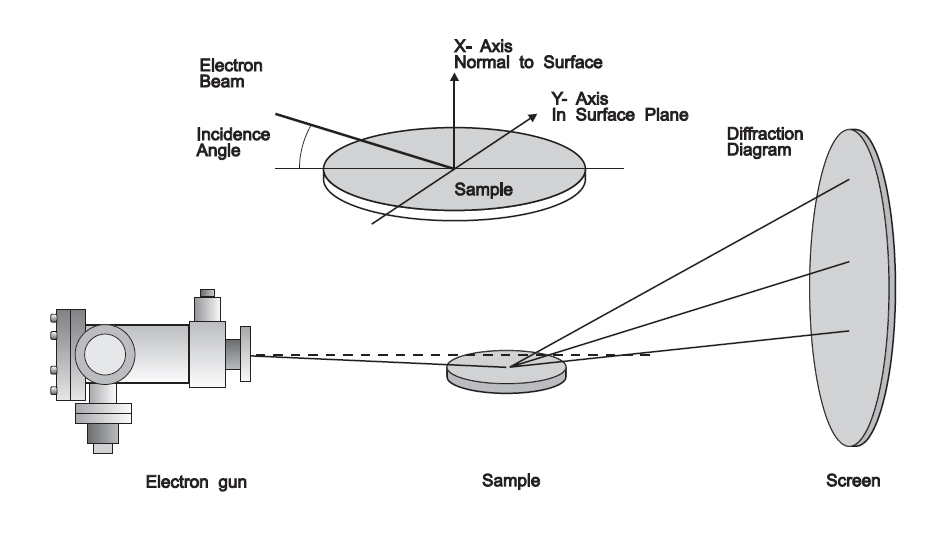
\includegraphics[width=1\textwidth]{images/setup1.png}
	\caption{Experimentální sestava běžně využívaná v růstových komorách MBE}
\end{figure}

Interpretace difrakčních obrazců v RHEED je zásadní pro pochopení morfologie povrchu. V případě dokonalé dvourozměrné mřížky se v reciprokém prostoru vytváří typické pruhové obrazce, zatímco přítomnost trojrozměrných ostrovů nebo teras vede ke vzniku bodových obrazců nebo tlumení difrakčních maxim. Díky analýze intenzitních oscilací těchto pruhů během depozice lze kvantitativně sledovat rychlost růstu jednotlivých monovrstev, což činí RHEED užitečným nástrojem při epitaxním růstu krystalů.\\

\begin{figure}[H]
	\centering
	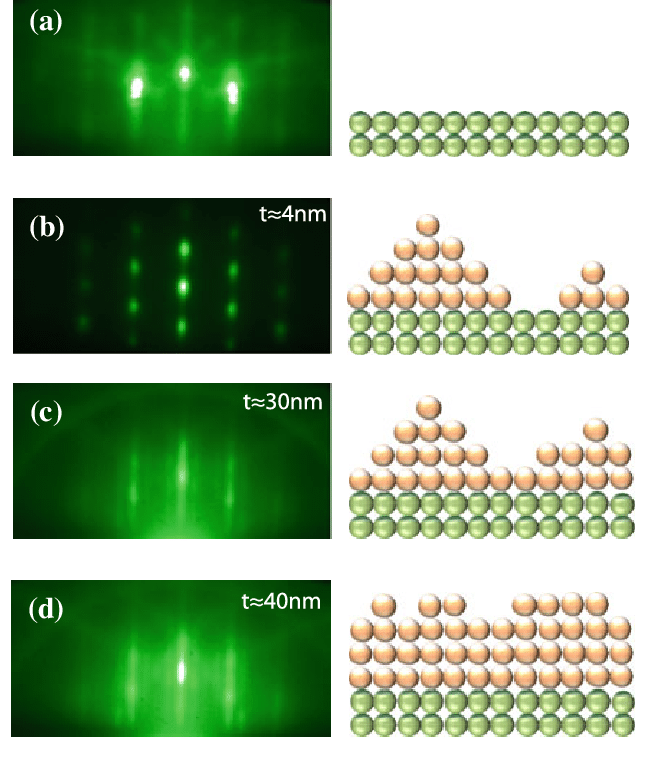
\includegraphics[width=0.8\textwidth]{images/interpretation.png}
	\caption{Příklady difrakčních vzorců RHEED a jejich korespondujícího interpretovaného obrazu ve formě uspořádání atomů}
\end{figure}

Význam RHEED v materiálových vědách je zejména při studiu tenkých vrstev polovodičových materiálů, kovových nanostruktur a oxidových vrstev. Tato metoda umožňuje nejen identifikaci symetrie povrchové mřížky, ale také detekci povrchových defektů, jako jsou kroky, dislokace nebo segregace nečistot. V kombinaci s dalšími analytickými metodami, například rentgenovou difrakcí (XRD) či rastrovací tunelovou mikroskopií (STM), poskytuje obraz o strukturách a vlastnostech povrchu na atomární úrovni. RHEED se stal nepostradatelným nástrojem hlavně při výzkumu polovodičových heterostruktur a kvantových definovaných nanostruktur. Ve spojení s MBE umožňuje optimalizaci růstových parametrů v reálném čase, čímž se zvyšuje kontrola nad kvalitou připravovaných vrstev. Z tohoto důvodu je široce využíván ve výzkumu materiálů pro \textbf{kvantovou elektroniku}, \textbf{spintroniku} či vývoj nových \textbf{dvourozměrných materiálů}, jako jsou topologické izolátory nebo grafenové deriváty.\\

\section{Aplikace RHEED a její struktura}
    V této kapitole bude rozebráno s čím aplikace pracuje a jednotlivé části aplikace.
\subsection{Kamera}
Pro snímání difrakčních vzorků jsme využili kameru \textbf{Player One Saturn-C}. Kamera disponuje CMOS snímačem s rozlišením 3856 x 2180 pixelů a velikostí pixelu 3.45 µm. To jí umožňuje detekovat i velmi malé detaily, nezbytný předpoklad při analýze difrakčních struktur.
    Dále má široký dynamický rozsah, tudíž není problém jak s intenzivními, tak slabými světelnými signály. Zároveň se zde nachází i optimalizovaná citlivost ve viditelném i blízkém infračerveném světle.
    Vysokorychlostní přenos dat zajišťuje rozhraní USB 3.0. To je důležité zejména pro sledování vzorku v reálném čase, znamená to žádné prodlevy a tudíž menší riziko zkažení vzorku.
    Výstup se zde nachází dvanáctibitový, tedy každý pixel je schopný zaznamenat až 4096 odstínů intenzity světla. Naprosto klíčový předpoklad v prostředí, kde i minimální rozdíl v intenzitě může nést důležité informace o struktuře vzorku.
    
    \begin{figure}[H]
    	\centering
    	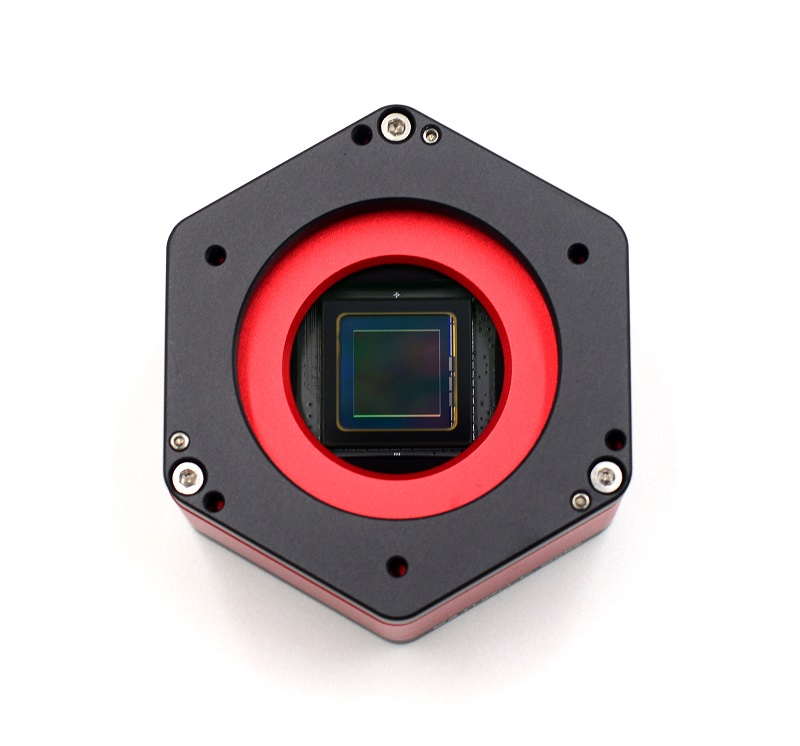
\includegraphics[width=0.8\textwidth]{images/saturn.png}
    	\caption{Použitá kamera Saturn-C, běžně používaná pro aplikace v astronomii nebo astrofyzice. Zde je vidět CMOS snímací detektor.}
    \end{figure}
    
\newpage
\subsubsection{Ovladač kamery}
S kamerou operuje soubor "opencv\_capture.py", který kameru za pomoci OpenCV inicializuje, konfiguruje a stará se o záznam snímků. Při spuštění je kamera inicializována a nastavena na požadované parametry. Při zdařilé inicializaci se otevírá datové úložiště, kde se každá relace ukládá do unikátního souboru ve složce cacheimg. To je adresář pro ukládání zachycených dynamických datasetů ve formátu h5py.\\

\begin{lstlisting}
class CameraInit:
    def __init__(self, width, height, initial_size):
        self.width = width
        self.height = height
        self.frame_index = 0
        self.dataset_size = initial_size  # Initial allocation size
        
        self.cache_folder = "cacheimg"
        os.makedirs(self.cache_folder, exist_ok=True)
        
        self.cap = cv2.VideoCapture(0)
        if not self.cap.isOpened():
            print("Failed to open camera.")
            return
        
        self.h5_file = h5py.File(
            os.path.join(self.cache_folder, f"dataset_{datetime.datetime.now().strftime('%d-%m-%Y_%H-%M-%S')}.h5"), "w"
        )

        self.image_dataset = self.h5_file.create_dataset(
            "arrays",
            shape=(self.dataset_size, self.width, self.height),
            maxshape=(None, self.width, self.height),
            dtype=np.uint16,
\end{lstlisting}
\captionof{lstlisting}{Inicializace kamery a ukládání dat do formátu HDF5}
\vspace{0.5cm}

Při ukončení záznamu je modul vybaven funkcemi zajišťujícími, že nedochází k úniku paměti nebo blokování systémových prostředků. Uzavírá se jak kamerové rozhraní tak soubory, čímž se předchází nechtěnému růstu souborů nebo vzniku chyb v již nasbíraných datech. Zároveň je vše uvedeno do stavu, kdy nic nebrání další bezproblémové inicializaci kamery.


\subsubsection{Ukládání, HDF5 formát a analýza snímků}
Ukládání a následná analýza difrakčních snímků jsou důležitými aspekty při zpracování dat. Pro efektivní správu a organizaci velkého množství získaných obrazových dat využíváme formát HDF5, který umožňuje strukturované ukládání dat s možností rozšiřování a optimalizace výkonu při čtení a zápisu. Veškeré snímky pořízené kamerou Player One Saturn-C jsou ukládány v binárním formátu s vysokou přesností, umožňující jejich následnou analýzu a vizualizaci v interaktivním prostředí aplikace.\\

HDF5 formát je tedy skvělou volbou pro organizaci a manipulaci s velkými objemy dat. HDF5 je hiearchycký souborový formát a umožňuje schraňování různých datových struktur v jednom souboru. V naší aplikaci je využíván pouze pro ukládání a organizaci snímků difrakčních vzorků, ale formát jako takový se dá využít i pro ukládání numerických simulacích nebo jiných měření. Dá se říci že je to systém menších souborů uvnitř jednoho většího binárního souboru. Organizování uvnitř formátu HDF5 jinak funguje velmi obdobně jako v běžném souborovém systému. Má tři hlavní složky: Skupiny, Datasety a Atributy. My pro ukládání snímků využíváme datasety, kde je každý snímek uložen jako matice hodnot intenzit.

Při inicializaci kamery se vytvoří nový soubor ve formátu HDF5, který slouží jako sklad pro všechny snímky pořízené v rámci jedné relace. Každý soubor je uložen v již zmíněné složce cacheimg, přičemž jeho název je generován dynamicky podle aktuálního data a času, aby bylo možné snímky jednoznačně identifikovat. Vytvořený dataset arrays je předalokován s definovanou počáteční kapacitou, čímž se minimalizuje latence při zápisu nových snímků. Díky funkci rozšiřitelnosti datasetu je také možné dynamicky alokovat další paměť v případě, že počet uložených snímků překročí původní alokaci. Tento proces probíhá automaticky a při dosažení limitu se dataset rozšíří o 1000 snímků.\\

\begin{lstlisting}
def capture_frame(self):
    ret, frame = self.cap.read()
    if not ret:
        print("Failed to capture frame.")
        return

    fr = cv2.cvtColor(frame, cv2.COLOR_BGR2GRAY)
    nfr = fr.astype(np.float64)

    if self.frame_index >= self.dataset_size:
        new_size = int(self.dataset_size + 1000)
        print(f"Resizing dataset from {self.dataset_size} to {new_size} frames...")
        self.image_dataset.resize(new_size, axis=0)
        self.dataset_size = new_size  

    self.image_dataset[self.frame_index] = nfr
    self.frame_index += 1

    return nfr
\end{lstlisting}
\captionof{lstlisting}{Zachycení a uložení snímku do datasetu}
\vspace{0.5cm}

Každý snímek je před uložením převáděn do stupňů šedi a volitelně může být normalizován s vysokou přesností pomocí 64bitových hodnot. Tento přístup je klíčový pro zachování detailů v intenzitě difrakčních vzorků, které by mohly být při běžném 8bitovém nebo 16bitovém ukládání ztraceny. Uložené snímky lze následně číst a zpracovávat v rámci dalších analýz, aniž by došlo ke snížení kvality záznamu. Vizualizace snímků probíhá v interaktivním grafickém prostředí s možností výběru konkrétních oblastí zájmu, více v kapitole "ROI a jejich správa". Pro zajištění plynulé vizualizace a analýzy je veškeré zpracování snímků realizováno v samostatném vláknu, které neblokuje hlavní běh aplikace. Díky tomu je možné sledovat změny v datech bez jakýchkoliv prodlev. Celý proces podporuje automatickou aktualizaci, přičemž uživatel může volit mezi manuálním a automatickým režimem, který průběžně zpracovává nové snímky.\\

Tento systém umožňuje nejen efektivní ukládání velkého objemu obrazových dat, ale také jejich pokročilou analýzu s využitím interaktivních nástrojů. Kombinace rychlého ukládání, dynamického rozšiřování datasetu a real-time vizualizace poskytuje uživateli výkonný nástroj pro studium difrakčních vzorků s vysokou přesností a flexibilitou.\\


\subsubsection{Zpracování obrazu}
V rámci vývoje softwaru pro analýzu RHEED snímků bylo nutné zajistit efektivní zpracování obrazu v reálném čase a jeho vizualizaci. K tomu je využita kombinace OpenCV pro získávání a předzpracování snímků a knihovny Silx pro jejich vykreslování. Důležitým prvkem je implementace Silx Plot2D s využitím OpenGL akcelerace, která umožňuje práci s obrazovými daty i při vysokém objemu snímků. To umožňuje uživateli provádět analýzu snímků bez výrazné latence.\\

Proces začíná snímáním obrazu pomocí kamery, přičemž data jsou získávána přes OpenCV a jak bylo zmíněno výše, jsou ihned převedena do odstínů šedi. Převod do monochromatické formy snižuje datovou náročnost a zjednodušuje další zpracování, především při analýze intenzity difrakčních vzorů. V této fázi může být prováděna také normalizace obrazu, což umožňuje optimalizaci kontrastu snímků. Po získání a úpravě obrazu je snímek odeslán do Silx Plot2D, který slouží jako vizualizační nástroj pro zobrazení jednotlivých snímků a dat. Zásadní výhodou tohoto řešení je využití OpenGL backendu, což umožňuje hardwarově akcelerované vykreslování. OpenGL významně snižuje nároky na procesor a umožňuje manipulaci se snímky i při vysokém objemu dat.\\

Pro plynulé zobrazení snímků je implementována vláknová správa aktualizace obrazu, která umožňuje přenos dat mezi OpenCV a Silx Plot2D. Tento přístup zajišťuje, že nově získané snímky jsou ihned přidány do vykreslovacího okna bez nutnosti pozastavení běhu aplikace. Snímky jsou přidávány pomocí asynchronních volání, aby GUI aplikace zůstalo responzivní i při dlouhodobém záznamu. Tím je zajištěno, že všechny vykreslovací operace jsou prováděny na GPU, čímž se významně snižuje zatížení CPU a umožňuje práci i při zobrazení několika snímků najednou. Díky tomu je možné nejen zobrazovat jednotlivé snímky, ale i provádět časovou analýzu sekvenčních dat, což je klíčové pro sledování dynamických změn v difrakčních vzorech.\\

\subsection{GUI aplikace}
GUI pro aplikaci RHEED je navrženo tak, aby poskytovalo uživatelsky přívětivé a intuitivní rozhraní pro vizualizaci obrazových dat a následnou analýzu. V GUI se může pracovat s kamerou, nastavením živého přenosu, vytvářením a úpravou ROI a analýzou dat. GUI je postaveno pomocí knihovny Silx což je nástavba na QTPY5

\subsubsection{Okno vizualizace}
Významným prvkem interaktivního uživatelského prostředí je okno vizualizace, které slouží k přehlednému zobrazení snímků a videa RHEED a jejich analýze. Tento modul zařizuje jak zobrazování snímků, správu ROI tak výpočty parametrů. Okno vizualizace je vytvořené s knihovnou Silx, která poskytuje užitečné nástroje pro zpracovávání a zobrazování dat.\\

Okno vizualizace se skládá z několika komponent: hlavní zobrazovací plocha, ROI manager, statistický panel, panel režimu aktualizace a Toolbar. Hlavní zobrazovací plocha zobrazuje aktuální snímek. Statistický panel vypočítává a zobrazuje parametry intenzity signálu pro vybrané ROI. Panel režimu aktualizace ovládá způsoby statistických výpočtů. Tyto dva panely spolu úzce souvisí a dodatečné informace k nim, ROI manageru a Toolbaru představíme v následujících podkapitolách. 

\subsubsection{Toolbar}
Toolbar obsahuje sadu tlačítek pro jednoduchou interakci s vizualizací obrazu a jeho přizpůsobením dle potřeb uživatele. Toolbar se nachází v horní části aplikace a poskytuje rychlý přístup k nástrojům pro navigaci, úpravu vzhledu a analýzu dat.\\

Pro manipulaci s obrazem lze využít tlačítkem lupy pro přiblížení vybrané oblasti, posuvník k pohybu po snímku bez změny měřítka. Vrátit všechny omyly v pohybu ve vizualizaci a oddálit přiblížení vizualizace je možné díky tlačítku přeškrtnuté lupy. Tlačítko "aspect ratio" umožňuje uživatelovi vybrat si mezi poměrem stran obrazu (možnost "keep aspect  ratio") a poměrem stran videa potažmo snímku (možnost "do not keep aspect ratio"). V Toolbaru se nachází nástroj pro změnu orientace osy Y. Uživatel zde má na výběr možnosti kdy osa roste buď nahoru (možnost "orient Y-axis upwards") a možnosti kdy osa klesá směrem dolů (možnost "orient Y-axis downwards").\\
\begin{figure}[H]
	\centering
	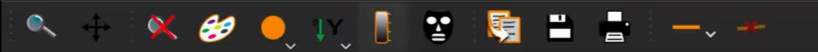
\includegraphics[width=0.8\textwidth]{images/Toolbar.png}
	\caption{Toolbar}
\end{figure}
Tlačítko pro kopírování obsahu vizualice zachycuje aktuální vizualizaci a ukládá snímek do schránky. Podobnou funkci zastává tlačítko s ikonou uložení, která uloží aktuální graf, obraz, nebo konkrétní křivku do souboru. Aplikace disponuje i tlačítkem pro tisk které při aktivaci umožní vytisknout aktuální graf a otevírá běžného správce tisku pro daný operační systém. Pro účely analýzy je zde i tlačítko pro horizontální přímkovou analýzu, které umožňuje výběr horizontálního profilu dat. Nakonec je zde tlačítko s přeškrtnutou čarou, které vymaže všechny aktuálně zobrazené přímkové profily.


\subsubsection{ROI}
ROI nebo také oblast zájmu slouží k vyhodnocování intenzity signálu v konkrétních částech snímku, tím umožňuje izolovat klíčové detaily pro další zpracování. ROI jsou základním nástrojem pro kvantitativní analýzu. Každá oblast je spravována ROI managerem, který se nachází v pravé části GUI jako dokovací okno. Ten zajišťuje jejich evidenci a propojení s analytickými funkcemi. Po přidání je ROI automaticky registrována do systému a propojena s nástrojem ROI Stats Widget, který umožňuje výpočet, vizualizaci statistik souvisejících s danou oblastí a ukazuje label (název), kind (typ), coordinates (souřadnice) a zároveň umožňuje ROI editovat nebo odstranit.\\

Proces přidávání ROI je umožněn prostřednictvím interaktivního uživatelského rozhraní obsaženého v ROI manageru. Uživatel má možnost manuálně definovat oblast na snímku pomocí myši a následně ji přizpůsobit podle požadavků analýzy. Po výběru ROI se její data okamžitě zapisují do interního systému aplikace. Každá ROI může být individuálně konfigurována, nebo-li uživatel může upravit její velikost, tvar a přesnou polohu ve snímku.\\

\begin{lstlisting}
	class _RoiStatsDisplayExWindow(qt.QMainWindow):
	def __init__(self, parent=None, mode=None):
	qt.QMainWindow.__init__(self, parent)
	self.plot = Plot2D(parent=self, backend="gl")
	self.setCentralWidget(self.plot)
	
	self._statsWidget = _RoiStatsWidget(parent=self, plot=self.plot)
	
	self._regionManager = RegionOfInterestManager(parent=self.plot)
	self._roiTable = RegionOfInterestTableWidget()
	self._roiTable.setRegionOfInterestManager(self._regionManager)
	
	self._roiToolbar = qt.QToolBar()
	self._roiToolbar.setIconSize(qt.QSize(16, 16))
	
	for roiClass in self._regionManager.getSupportedRoiClasses():
	self._roiToolbar.addAction(self._regionManager.getInteractionModeAction(roiClass))
	
	modeSelectorAction = RoiModeSelectorAction()
	modeSelectorAction.setRoiManager(self._regionManager)
	
\end{lstlisting}
\captionof{lstlisting}{Vizualizace, výběr a analýza ROI}
\newpage
\begin{figure}[H]
	\centering
	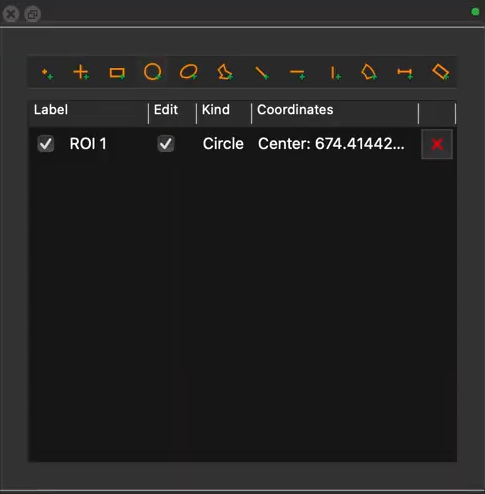
\includegraphics[width=0.5\textwidth]{images/ROIManager.png}
	\caption{ROI manager}
\end{figure}

Aplikace podporuje různé tvary, mezi které patří předdefinované obdélníkové, eliptické nebo polygony volně definované uživatelem, což poskytuje vysokou flexibilitu při analýze. Každá přidaná oblast je evidována ve správci ROI, kde je možné ji přejmenovat, duplikovat, nebo odstranit, čímž se usnadňuje organizace a porovnávání různých částí snímku.\\

Díky automatickému režimu aktualizace je jakákoli změna ROI okamžitě reflektována ve výpočtech a vizualizaci dat. Pokud uživatel preferuje manuální režim, je možné aktualizaci řídit pomocí ručně spouštěných výpočtů pro lepší kontrolu nad vyhodnocením výsledků. Všechny změny ROI jsou uchovávány po dobu analýzy a lze je dynamicky měnit podle potřeby.

\subsubsection{Statistický panel}
Statistická panel slouží k analýze dat v rámci jednotlivých ROI. Implementován je s pomocí ROIStatsWidget, který propojuje ROI manager s výpočetními funkcemi a poskytuje přehled statistik vypočítaných pro jednotlivé ROI. Hlavním údajem, který je klíčovým pro analýzu difrakčních obrazců je průměrná hodnota vypočtena z celkové plochy pixelů, které jsou obsaženy ve zvoleném ROI.
\begin{figure}[H]
    \centering
    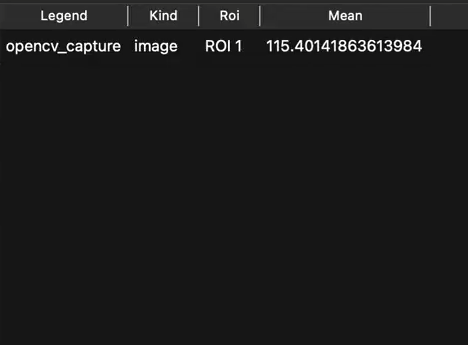
\includegraphics[width=0.5\textwidth]{images/StatistickyPanel.png}
    \caption{Statistický panel}
\end{figure}

\subsubsection{Panel režimu aktualizace}
Panel režimu aktualizace slouží k ovládání způsobu, jakým se aktualizují statistické výpočty. Uživateli je v něm umožněno přepínat mezi dvěma režimy aktualizace. V automatickém režimu jsou statistiky přepočítávány průběžně bez zásahu uživatele, zatímco v manuálním režimu se aktualizace provede pouze po stisknutí tlačítka "update".\\

\newpage
\section{Zdroje}
%\textbf{h5py} - \cite{h5pyDocs}\\
%\textbf{Matplotlib} - \cite{matplotlibDocs}\\
%\textbf{Numpy} - \cite{numpyDocs}\\
%\textbf{OpenCV} - \cite{opencvDocs}\\
%\textbf{Silx} - \cite{silxDocs}\\
%\textbf{Player One SDK} - \cite{PlayerOneSDK}\\
%\textbf{RHEED} - \cite{RHEED}\\
%\textbf{HDF5} - \cite{WhatIsHDF5}\\
\nocite{*}

\printbibliography
\end{document}